\documentclass[dvisvgm,tikz]{standalone}

\usepackage[sfdefault]{inter}
\usetikzlibrary{shapes.geometric, arrows.meta, positioning, calc, fit, decorations.pathmorphing}

%%%%%%%%%%%%%%%%%%%%%%%%%%%%%%%%%%%%%%%%%%%%%%%%%%%
%Colors
% Warm gray to turquoise
\definecolor{warm_gray}{RGB}{128, 120, 115}
\definecolor{sage_gray}{RGB}{110, 125, 120}
\definecolor{pewter}{RGB}{91, 112, 114}
\definecolor{slate_blue}{RGB}{72, 107, 115}
\definecolor{steel_teal}{RGB}{53, 118, 125}
\definecolor{teal}{RGB}{27, 136, 140}
\definecolor{deep_aqua}{RGB}{15, 152, 155}
\definecolor{peacock_blue}{RGB}{0, 167, 171}
\definecolor{blue_green}{RGB}{0, 181, 185}
\definecolor{turquoise}{RGB}{0, 195, 200}

\definecolor{mygray}{gray}{0.9}

% Match our established color scheme
\definecolor{atoken}{RGB}{255, 152, 0}        % Orange for A token
\definecolor{gtoken}{RGB}{76, 175, 80}        % Green for G token
\definecolor{mainblue}{RGB}{74, 144, 226}     % Blue for A classes
\definecolor{maingreen}{RGB}{102, 187, 106}   % Light green for G classes
\definecolor{timegray}{RGB}{158, 158, 158}    % Gray for time component
%%%%%%%%%%%%%%%%%%%%%%%%%%%%%%%%%%%%%%%%%%%%%%%%%%%

\def \G {\textbf{G}}
\def \A {\textbf{A}}
\def \Q {\textbf{Q}}
\def \C {\textbf{C}}
\def \CC {\textbf{C*}}
\def \KA {\textbf{KLIMA}}
\def \KG {\textbf{KlimaX}}

\def \AG {$\overline{\textbf{AG}}$}
\def \AQ {$\overline{\textbf{AQ}}$}

\begin{document}
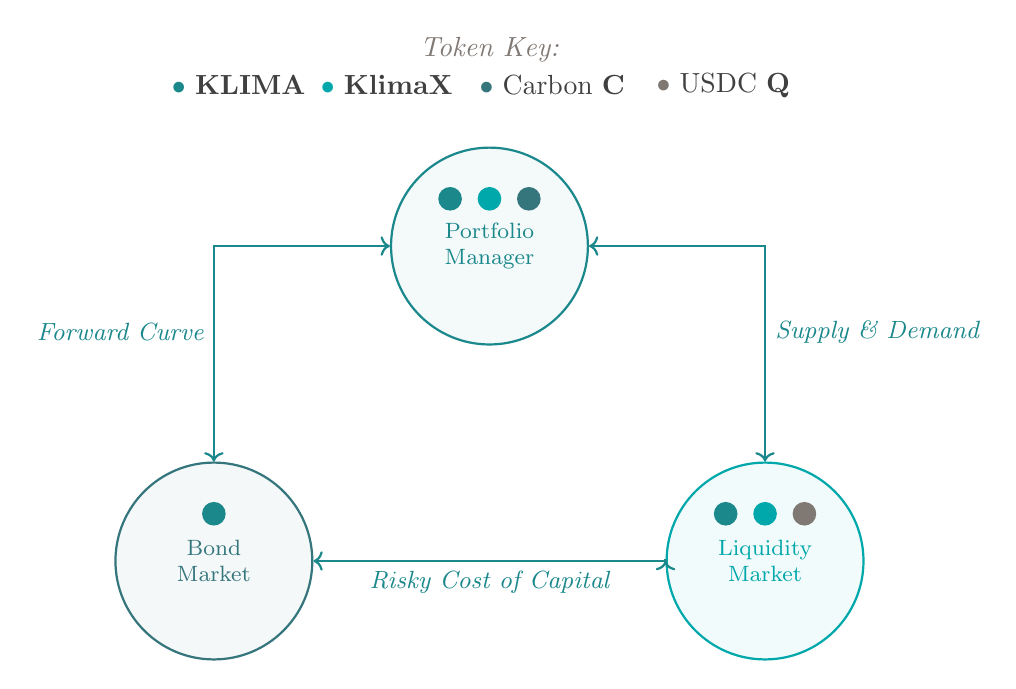
\begin{tikzpicture}[
    % Define the market node style
    market/.style={
        circle,
        minimum size=2.5cm,
        thick,
        draw=#1,
        fill=#1!05,
        text=#1,
        align=center,
        font=\footnotesize
    },
    % Connection style
    connect/.style={
        <->,
        thick,
        #1
    },
    % Token dot style
    token/.style={
        circle,
        fill=#1,
        minimum size=0.3cm,
        inner sep=0pt
    }
]

\node[text=warm_gray, align=left, font=\itshape] at (0,6.5) {Token Key:};
\node[text=darkgray, align=left] at (-3.1845,6.0435) {\textcolor{teal}{$\bullet$} \KA{}};
\node[text=darkgray, align=left] at (-1.3044,6.0486) {\textcolor{peacock_blue}{$\bullet$} \KG{}};
\node[text=darkgray, align=left] at (0.7979,6.0429) {\textcolor{steel_teal}{$\bullet$} Carbon \C{}};
\node[text=darkgray, align=left] at (2.971,6.0346) {\textcolor{warm_gray}{$\bullet$} USDC \Q{}};

% Position the three markets
\node[market=teal] (aam) at (0,4) {Portfolio \\ Manager};

\node[market=steel_teal] (bond) at (-3.5,0) {Bond\\Market};
\node[market=peacock_blue] (liquidity) at (3.5,0) {Liquidity\\Market};

\draw[connect=teal] (aam.west) -| node[pos=0.7, left, text=teal, font=\small\itshape] {Forward Curve}  (bond.north);

\draw[connect=teal] (aam.east) -| node[pos=0.7, right, text=teal, font=\small\itshape] {Supply \& Demand}  (liquidity.north);

\draw[connect=teal] (bond.east) -| node[pos=0.25, below, text=teal, font=\small\itshape] {Risky Cost of Capital}  (liquidity.west);


% Add tokens to AAM
\node[token=teal] at (-0.5,4.6) {};
\node[token=peacock_blue] at (0,4.6) {};
\node[token=steel_teal] at (0.5,4.6) {};

% Add token to Bond Market
\node[token=teal] at (-3.5,0.6) {};

% Add tokens to Liquidity Market
\node[token=teal] at (3.0,0.6) {};
\node[token=peacock_blue] at (3.5,0.6) {};

\node[token=warm_gray] at (4.0,0.6) {};

\end{tikzpicture}
\end{document}
